\documentclass[11pt,a4paper]{article}
\usepackage[a4paper,hmargin=1in,vmargin=1in]{geometry}
\usepackage{pgfplots}
\pgfplotsset{compat=1.17}

\usepackage[british]{babel}
\usepackage[utf8]{inputenc}
\usepackage[T1]{fontenc}

\usepackage{stddoc}
\usepackage{lipsum}
\usepackage{subcaption}

\usepackage{listings}
\lstloadlanguages{Matlab}

\newcommand{\plus}{{\texttt{+}}}
\renewcommand{\Re}{\operatorname{Re}}
\renewcommand{\Im}{\operatorname{Im}}
\newcommand{\fourier}[3]{\mathcal{F}_{#1}\!\left[#2\right]\!\left(#3\right)}
\newcommand{\ifourier}[3]{\mathcal{F}^{-1}_{#1}\!\left[#2\right]\!\left(#3\right)}


\begin{document}

\pagenumbering{arabic}

% Header
\begin{center}
    {\LARGE\textbf{B2M17CADA - Project I}}\\[3mm]
    \begin{minipage}{0.4\textwidth}
        \begin{flushleft}
            \textsc{\today}
        \end{flushleft}
    \end{minipage}
    ~
    \begin{minipage}{0.4\textwidth}
        \begin{flushright}
            \textsc{Martin Šimák}
        \end{flushright}
    \end{minipage}
    \noindent\rule{14.5cm}{0.4pt}
\end{center}

\paragraph{Task} \emph{Analysis of a stripline using finite differences}\\
Determine the properties of a shielded coplanar stripline depicted in figure~\ref{fig:task-geometry} designed on a suspended dielectric substrate ($h = 1~\mathrm{mm}$, $\epsilon_r = 3.05$) using finite differences and the method of successive over-relaxation. Find the strip's width $w$ and gap $g$ between the strips so that the characteristic impedance is $Z_0 = 50~\mathrm{\Omega}$. The distance of the shielding walls from the strips should be larger than $20h$ to ensure that the line's impedance is not affected by finite dimensions.
\begin{figure}[!ht]
    \centering
    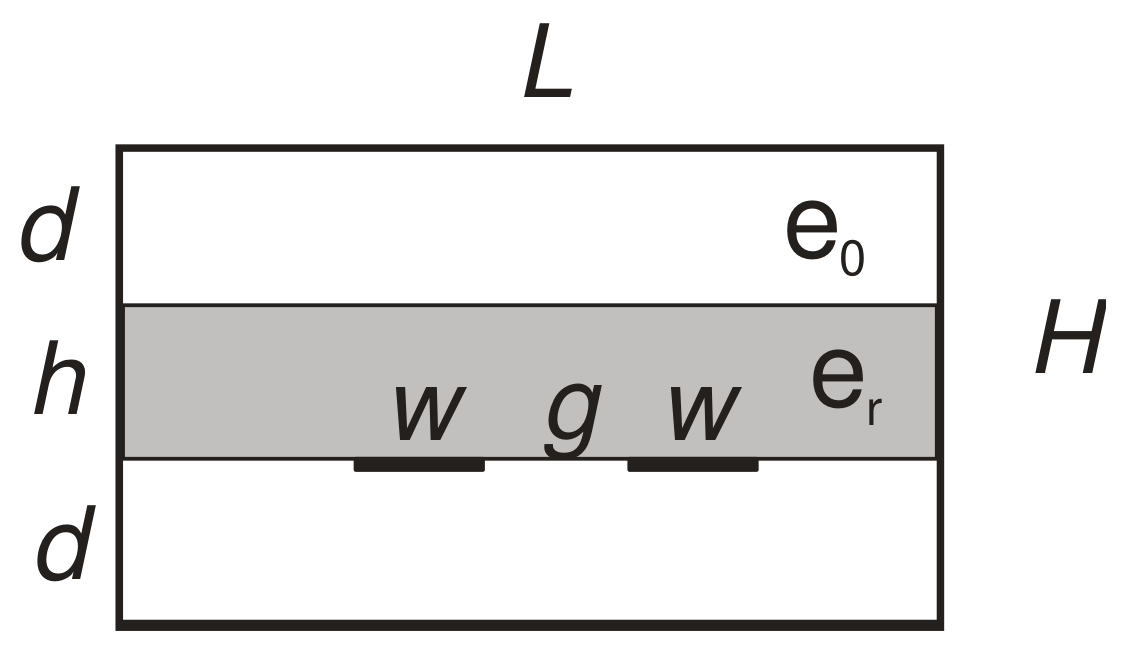
\includegraphics[width=.4\textwidth]{src/task-geometry.png}
    \caption{Task geometry}
    \label{fig:task-geometry}
\end{figure}

\begin{enumerate}[label=(\alph*)]
    \item Illustrate equipotencial countours and the distribution of electric field.
    \item Evaluate the capacity per unit length and the characteristic impedance $Z_0$.
    \item Plot the value of $Z_0$ as a function of number of iterations.
    \item Find the charge density on a strip.
    \item Determine numerically optimal value of the relaxation coefficient $\alpha$. Compare with the analytical solution
    \begin{align}
        \label{eq:alpha-analytical-solution}
        \alpha = \frac{8-\sqrt{64-16r^2}}{r^2},
    \end{align}
    where $r = \cos(\pi/N_x) + \cos(\pi/N_y)$ and $N_x \times N_y$ are the dimensions of the discrete mesh.
\end{enumerate}

\newpage\section{Theoretical introduction}
Generally speaking, finite-difference methods are a class of numerical analysis techniques used for solving differential equations. This is done via breaking the computational domain (spatial or temporal in most cases) into a finite number of steps which allows for the replacement of differential operators, such as derivatives, with differences.

Methods based on finite differences are very useful for converting nonlinear differential equations into a system of linear equations which can be efficiently solved by matrix algebra techniques, e.g. Gauss-Seidel method and its variants. Since these linear algebra computations are very efficiently implemented in modern computers, finite-difference methods are one of the most common approaches to the numerical solution of differential equations.

In our case, we use finite differences to approximate the differential operator from the Gauss's law which has the integral form of
\begin{align}
    \label{eq:gauss-3d}
    \oint_S \epsilon \vec E \cdot \mathrm d \vec S &= Q.
\end{align}
However, in a plane, this equation simplifies to
\begin{align}
    \label{eq:gauss-2d}
    \oint_C \epsilon \vec E \cdot \mathrm d \vec c &= q_l,
\end{align}
where $C$ is the bounding curve of the area $S$ used in the full form~\ref{eq:gauss-3d} and $q_l = Q/l$ is the line charge density. Furthermore, assuming electrostatic (irrotational) field, we can put $\vec E = -\grad \varphi$ simplifying equation~\ref{eq:gauss-2d} even further into the form of
\begin{align}
    -\oint_C \epsilon \, \grad \varphi \cdot \mathrm d \vec c &= q_l,
\\
    \label{eq:gauss-final}
    \oint_C \epsilon \pder{\varphi}{n} \; \mathrm d c &= -q_l.
\end{align}

\noindent%
\begin{minipage}{.6\textwidth}
    The integrand in~\ref{eq:gauss-final} represents the flux of electric field
    \begin{align*}
        \mathrm d \Psi = \epsilon \pder{\varphi}{n} \; \mathrm d c
    \end{align*}
    through the curve $C$ enclosing the node. This situation is depicted in figure~\ref{fig:cell} and can be expressed as
    \begin{align*}
        \Psi_1 &= \epsilon_1 \frac{\varphi_1-\varphi_0}{h} \frac h2 + \epsilon_2 \frac{\varphi_1-\varphi_0}{h} \frac h2,
    \\
        \Psi_2 &= \epsilon_1 \frac{\varphi_2-\varphi_0}{h} h,
    \\
        \Psi_3 &= \epsilon_1 \frac{\varphi_3-\varphi_0}{h} \frac h2 + \epsilon_2 \frac{\varphi_3-\varphi_0}{h} \frac h2,
    \\
        \Psi_4 &= \epsilon_2 \frac{\varphi_4-\varphi_0}{h} h.
    \end{align*}
\end{minipage}\hfill\begin{minipage}{.35\textwidth}
    \centering
    \captionsetup{type=figure}
    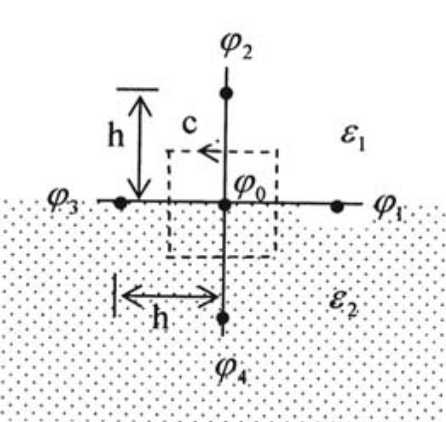
\includegraphics[width=\textwidth]{src/cell.png}
    \captionof{figure}{Modified Gauss's law around a node of potential $\varphi_0$}
    \label{fig:cell}
\end{minipage}

\noindent%
However, from Gauss's law, we know that $\Psi_1 + \Psi_2 + \Psi_3 + \Psi_4 = 0$ because there is no charge present. This yields
\begin{align}
    \label{eq:step1}
    \frac{\epsilon_1+\epsilon_2}{2} \varphi_0 = \frac 14 \(\frac{\epsilon_1+\epsilon_2}{2}\varphi_1 + \epsilon_1\varphi_2 + \frac{\epsilon_1+\epsilon_2}{2}\varphi_3 + \epsilon_2\varphi_4\).
\end{align}
This final equation serves as the finite-difference approach to solving the electrostatic potential distribution in the \emph{free nodes} of the configuration, i.e., nodes not in the electrodes, including planar dielectric interfaces. In the case of the stripline, $\epsilon_1 = \epsilon_0$, $\epsilon_2 = \epsilon_r \epsilon_0$ and we keep constant feeding voltage connected to the strips (electrodes) in every iteration. The rest of the procedure is successive over-relaxation.

The second part of our calculation involves charge density from which we can extract information about the capacity per unit length and the characteristic impedance.

\noindent%
\begin{minipage}{.6\textwidth}
    Again, we utilize the equation~\ref{eq:gauss-final} which has a non-zero right-hand side now because the curve encompasses the charges strips. The situation is similar to a one-electrode problem in figure~\ref{fig:electrode}.
\end{minipage}\hfill\begin{minipage}{.35\textwidth}
    \centering
    \captionsetup{type=figure}
    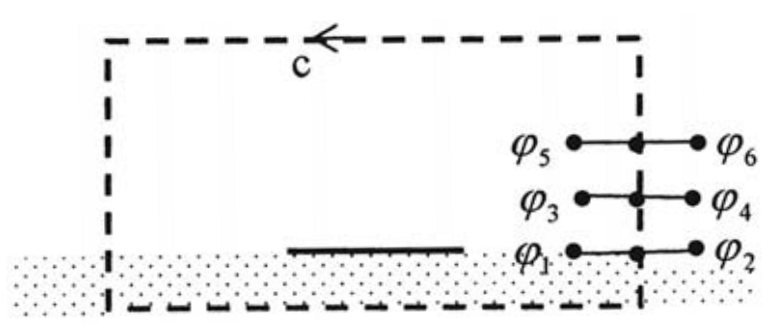
\includegraphics[width=\textwidth]{src/electrode.png}
    \captionof{figure}{Modified Gauss's law around a charged electrode}
    \label{fig:electrode}
\end{minipage}

\noindent%
Using this illustration, we can write
\begin{align}
    \label{eq:step2}
    \Psi = \epsilon_1 \frac{\varphi_2-\varphi_1}{2h} \frac h2 + \epsilon_2 \frac{\varphi_2-\varphi_1}{2h} \frac h2 + \epsilon_2 \frac{\varphi_4-\varphi_3}{2h}h + \epsilon_2 \frac{\varphi_6-\varphi_5}{2h}h + \cdots &= q_l
\end{align}
which serves as the main computational formula for further results.

\newpage\section{Implementation}
The code below represents the core computational loop. The first step is to perform the relaxation of electric potential using~\ref{eq:step1} over the whole mesh. Then, for a given iteration, the script computes charge density using~\ref{eq:step2}. Results are saved for every iteration in order to track the evolution of impedance values. This number is highly dependent on the threshold value which breaks the loop once the previous relaxation step hasn't improved the solution by at least the threshold value.
\begin{lstlisting}[language=Matlab]
while Rmax > 1e-3
    iter = iter + 1;
    % Step 1: SOR method
    for j = 2:Nx-1
    for i = 2:Ny-1
        if i == IF1
            R(i,j) = (eps_r*V(i+1,j)+1*V(i-1,j)+er_avg*V(i,j-1)+ ...
                er_avg*V(i,j+1))/4/er_avg-V(i,j); 
        elseif i == IF2
            R(i,j) = (1*V(i+1,j)+eps_r*V(i-1,j)+er_avg*V(i,j-1)+ ...
                er_avg*V(i,j+1))/4/er_avg-V(i,j); 
        else
            R(i,j) = (V(i+1,j)+V(i-1,j)+V(i,j-1)+V(i,j+1))/4-V(i,j);
        end
            V(i,j) = V(i,j)+alpha*R(i,j);
        V(IF1-1,Nx/2-g/2-w/2:Nx/2-g/2+w/2) = V0;
        V(IF1-1,Nx/2+g/2-w/2:Nx/2+g/2+w/2) = V0;
    end
    end
    Rmax = max(max(R));
    % Step 2: numerical evaluation of the intergral
    qA = 0; qB = 0; qC = 0; qD = 0;
    for i=top:1:bottom
        if i < IF1
            qA = qA + eps_r*(V(i,left+1) - V(i,left-1))/2;
            qC = qC + eps_r*(V(i,right-1) - V(i,right+1))/2;
        elseif i == IF1
            qA = qA + er_avg*(V(i,left+1) - V(i,left-1))/2;
            qC = qC + er_avg*(V(i,right-1) - V(i,right+1))/2;
        else
            qA = qA + (V(i,left+1) - V(i,left-1))/2;
            qC = qC + (V(i,right-1) - V(i,right+1))/2;
        end
    end
    for j=left:1:right
            qB = qB + (V(bottom+1,j) - V(bottom-1,j))/2;
            qD = qD + eps_r*(V(top-1,j) - V(top+1,j))/2;
    end
    Q(iter) = eps_0*(qA + qB + qC + qD);
end
C = Q/(V0-Vgnd);
Z = 1./(c*C);
\end{lstlisting}

\section{Results}
Figure~\ref{fig:output-field} shows the resultant electric field distribution, whereas in figure~\ref{fig:output-z0-alpha17}, I have inspected the evolution of characteristic throughout the run.
\begin{figure}[!ht]
    \centering
    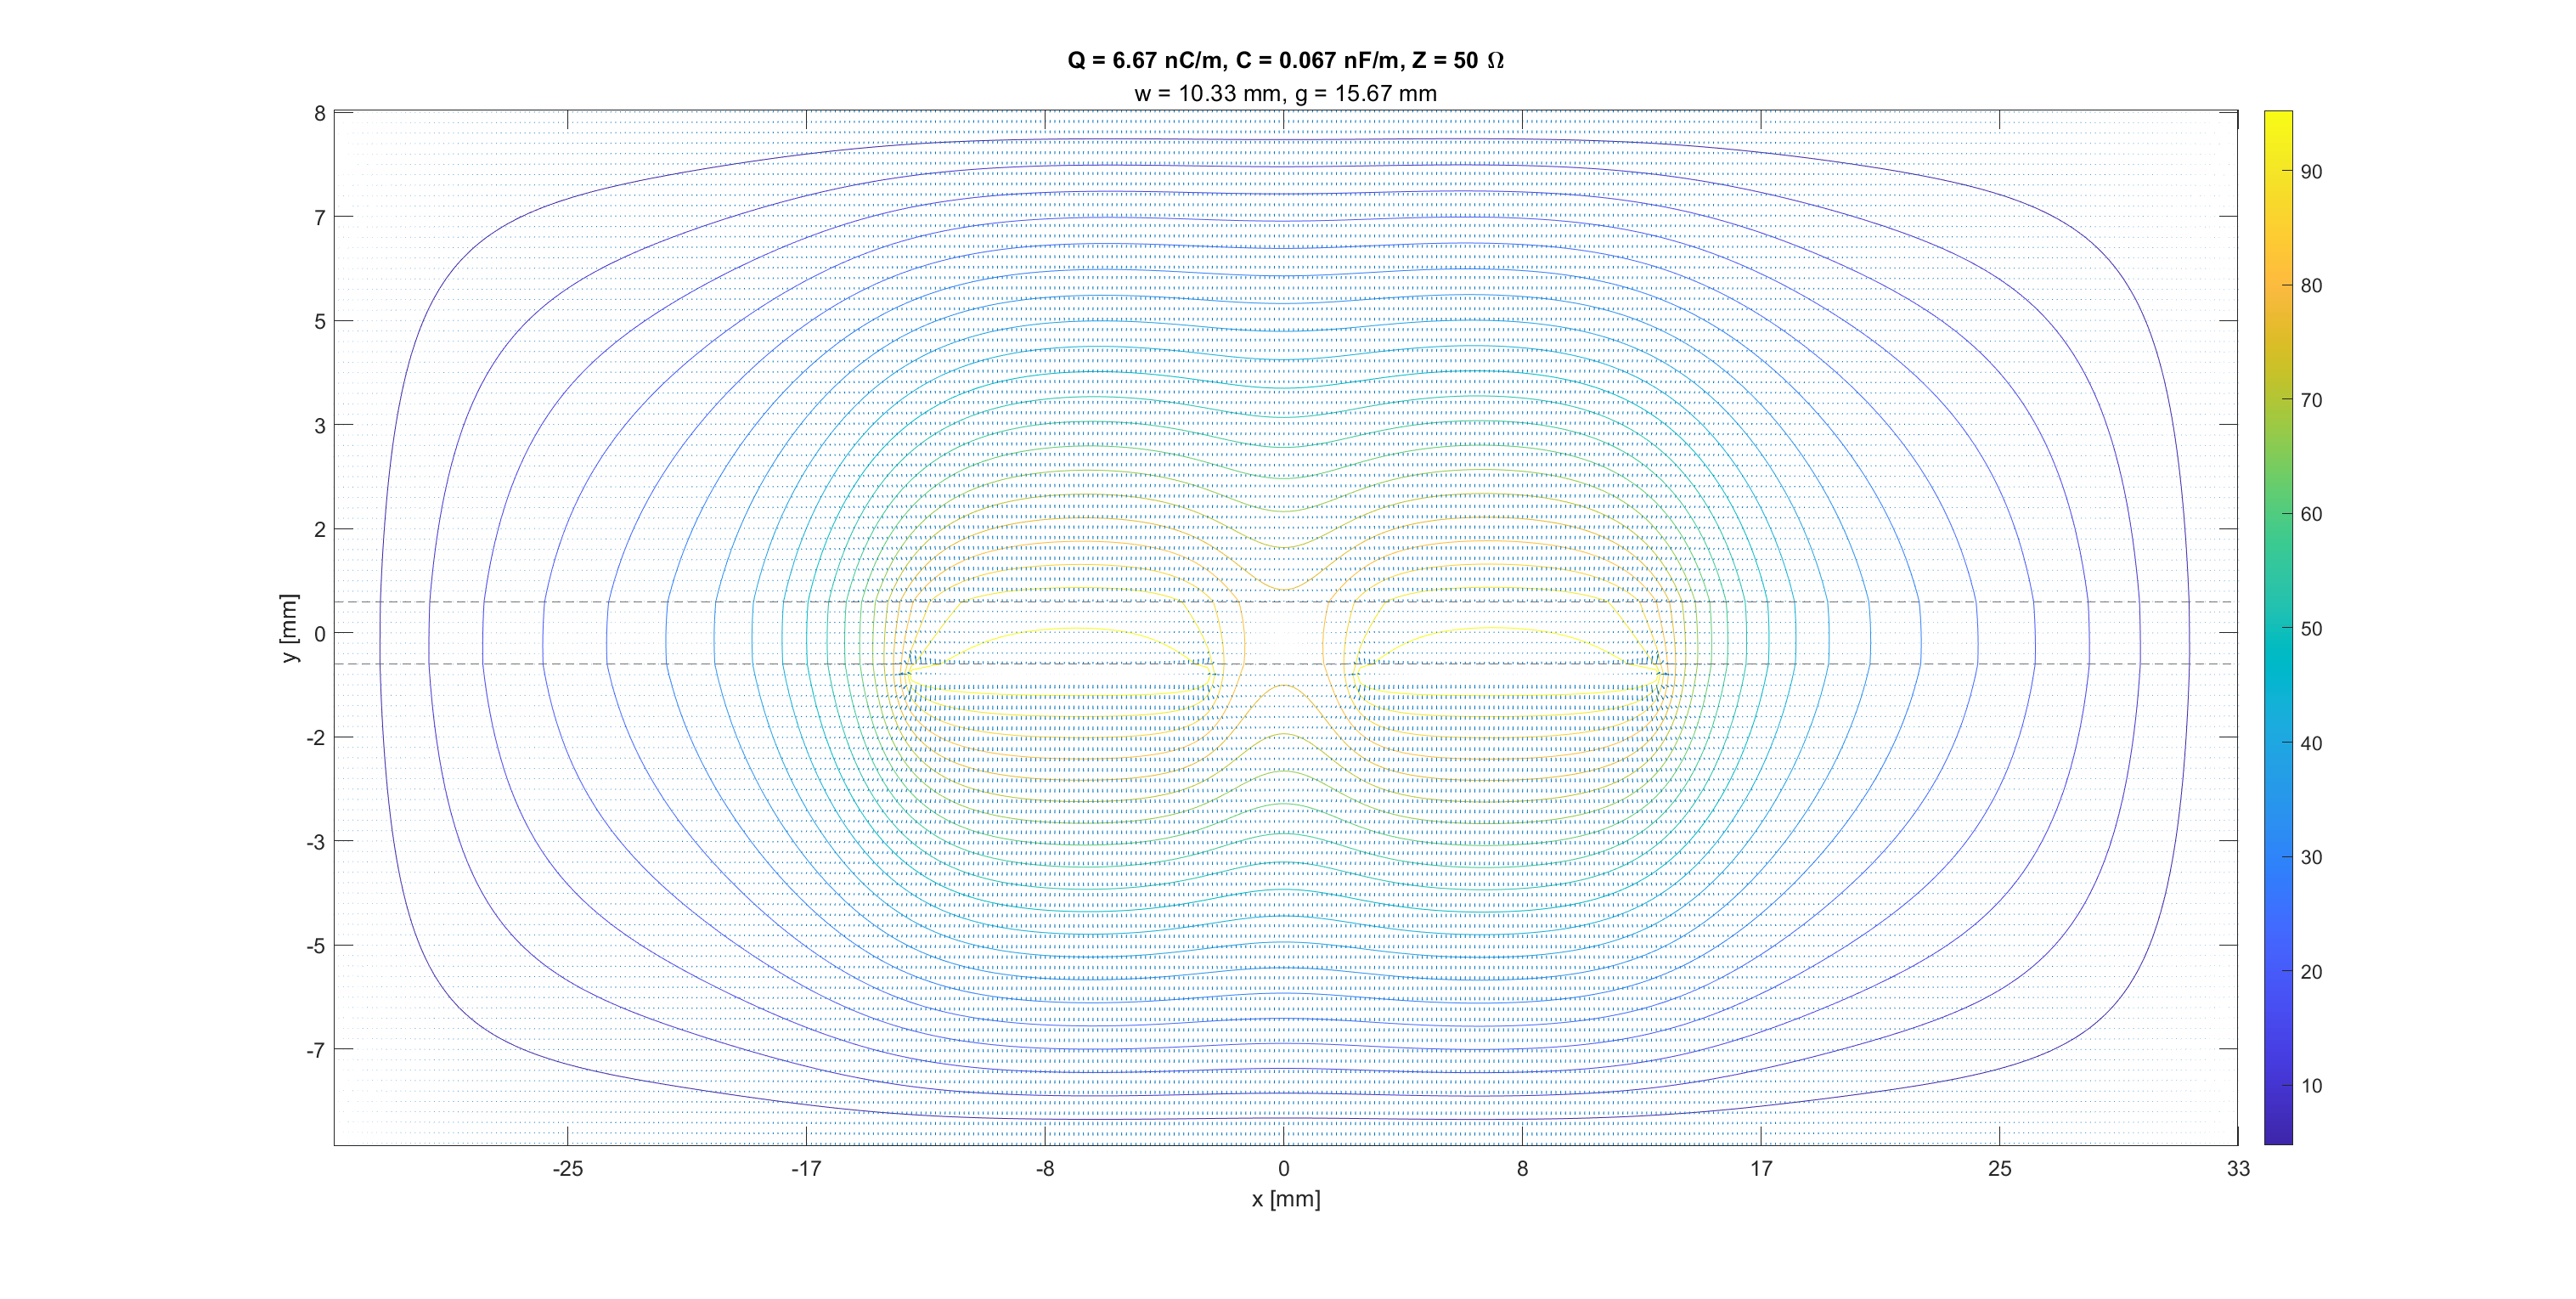
\includegraphics[width=\textwidth]{src/output_field_alpha1-7.eps}
    \caption{Output field}
    \label{fig:output-field}
\end{figure}
\begin{figure}[!ht]
    \centering
    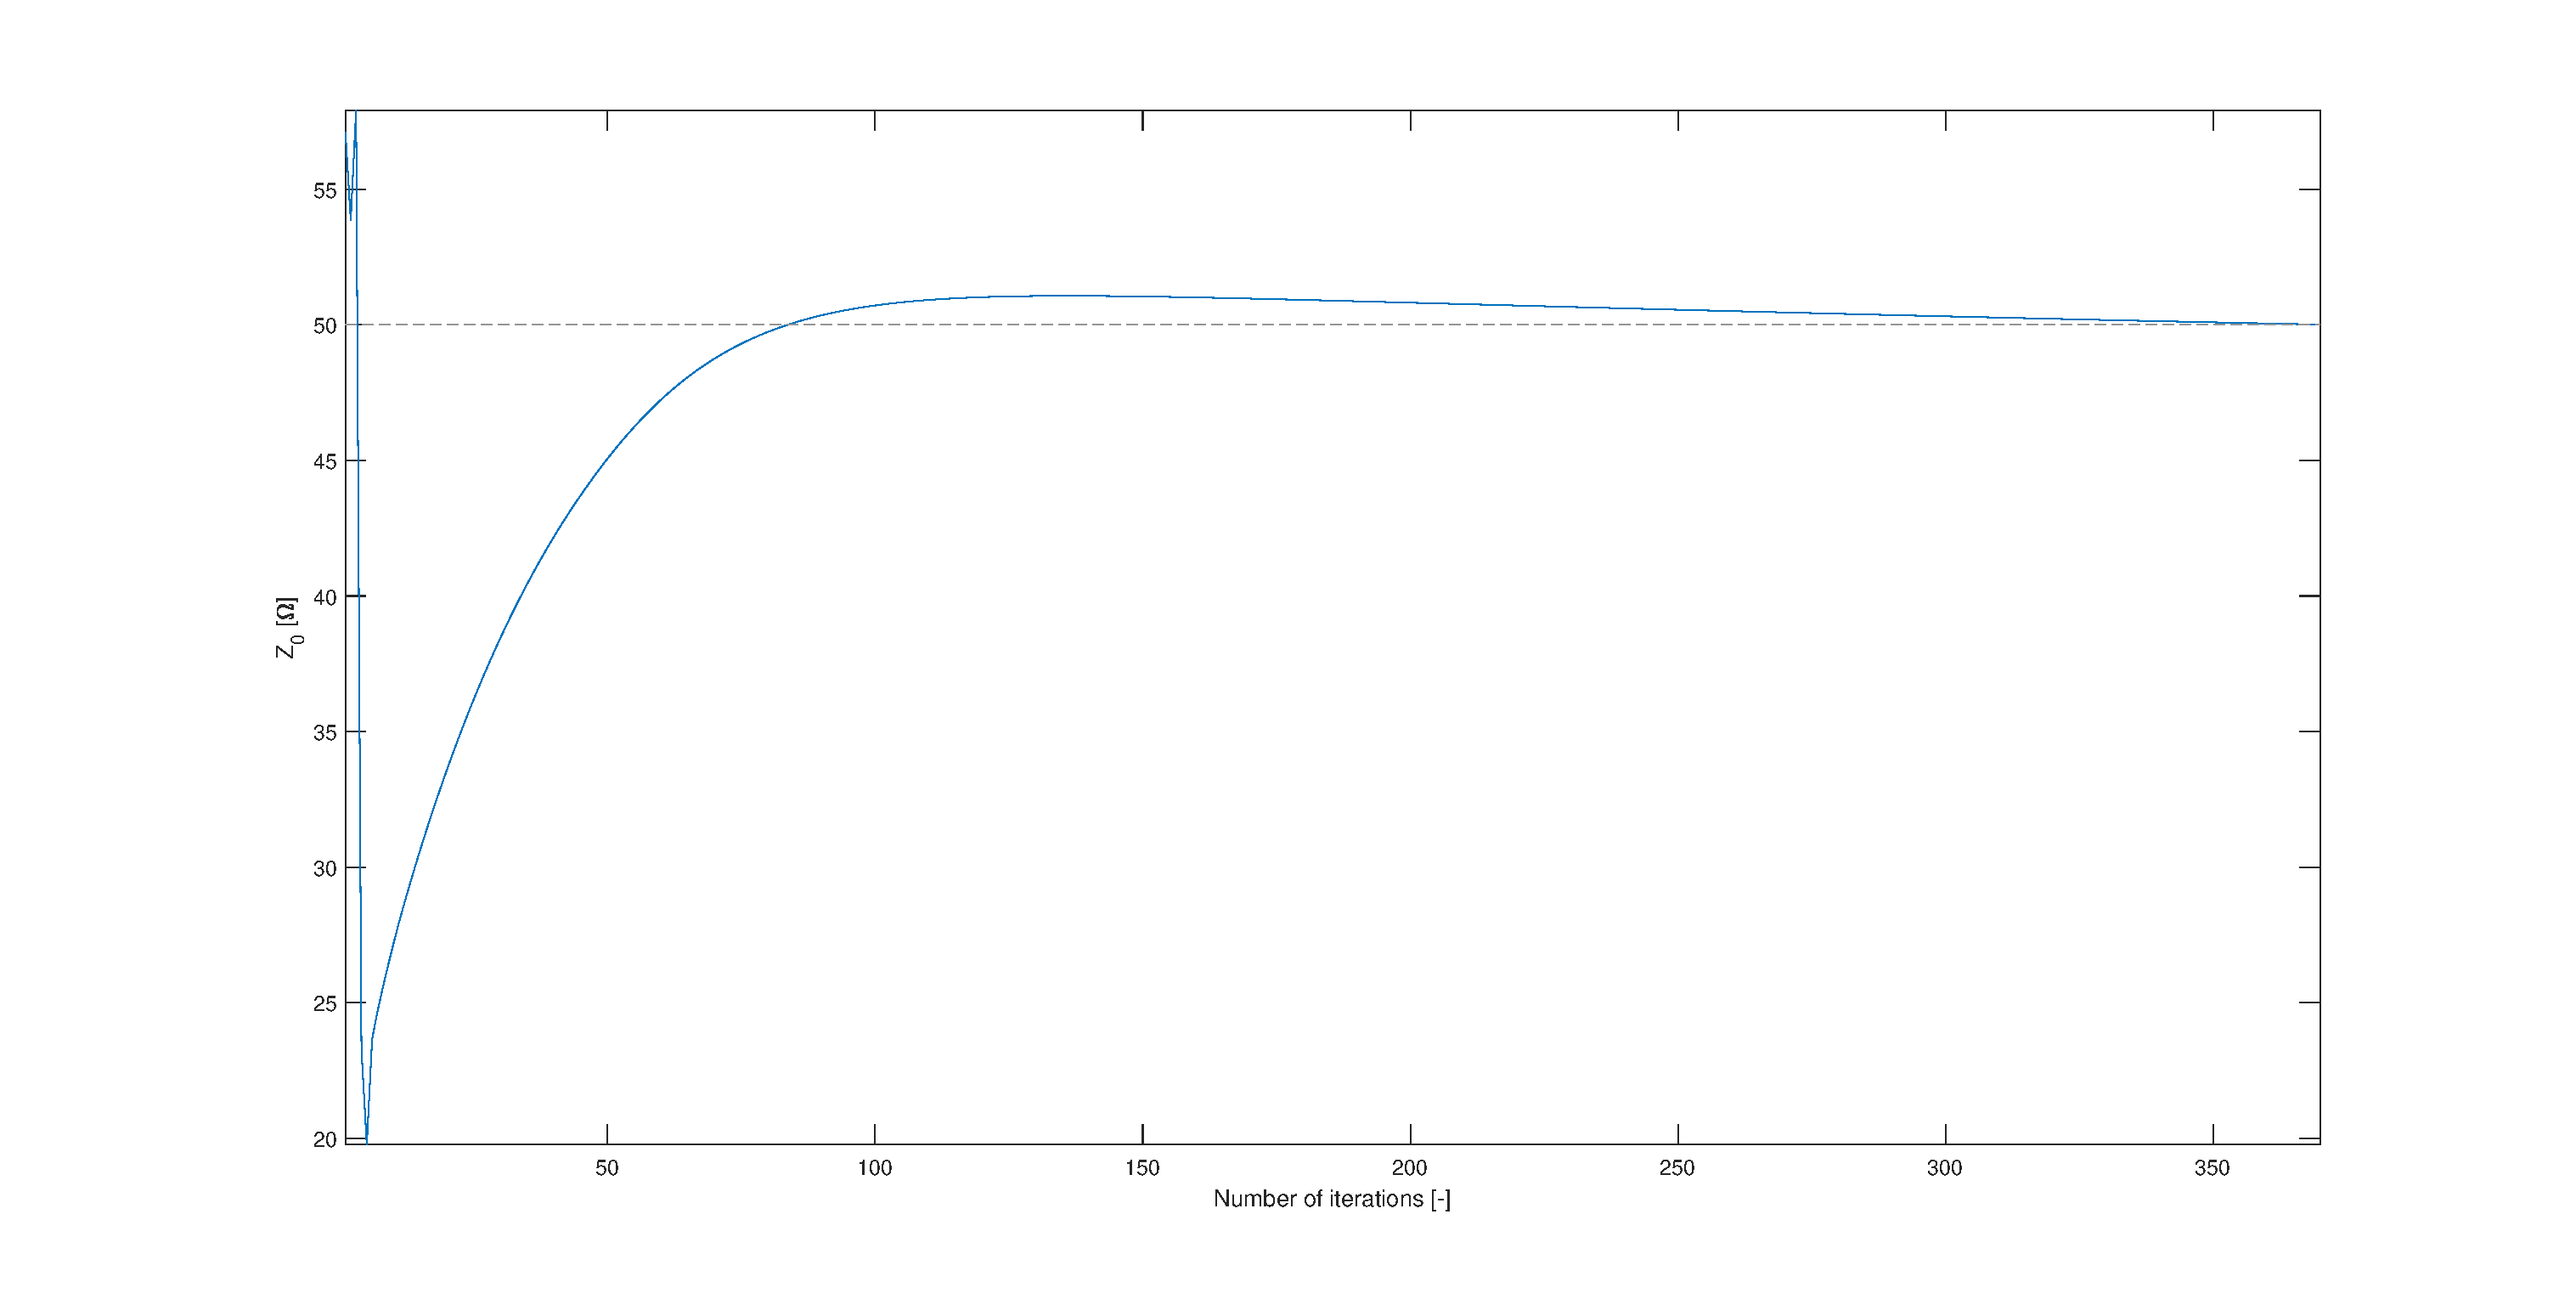
\includegraphics[width=\textwidth]{src/output_z0_alpha1-7.eps}
    \caption{Evolution of the characteristic impedance over iterations}
    \label{fig:output-z0-alpha17}
\end{figure}

Numerical determination of the optimal value of $\alpha$ yielded the number $1.91$ which is fairly compliant with the analytical solution of $\alpha_0 = 1.96$.

\end{document}
